\section{Vaccination}

\subsection{Model structure}
In this application we introduced separate strata to the model for vaccinated an unvaccinated individuals.
All model compartments are replicated into three categories:

\begin{itemize}
	\item Unvaccinated persons
	\item Persons who have only received one dose of vaccination
	\item Persons who have received two doses of vaccination (i.e. the full course)
\end{itemize}

Note that the model does not contain structure to represent different types of vaccination, despite different schedules likely having somewhat different characteristics.
This decision was made in the interest of parsimony, given the extreme level of complexity that the model structure has reached in relation to other features.

\subsection{Vaccination process}
The process of vaccination is only applied to the susceptible and recovered compartments and not to any of the compartments representing current active infection.
Transition flows are applied to move persons from the unvaccinated compartments to the one-dose compartments according to the history of vaccination roll-out.
The transition flow from the one dose stratum to the two dose stratum is then applied with a rate equal to the reciprocal of the average delay between first and second dose.

\begin{figure}[ht]
    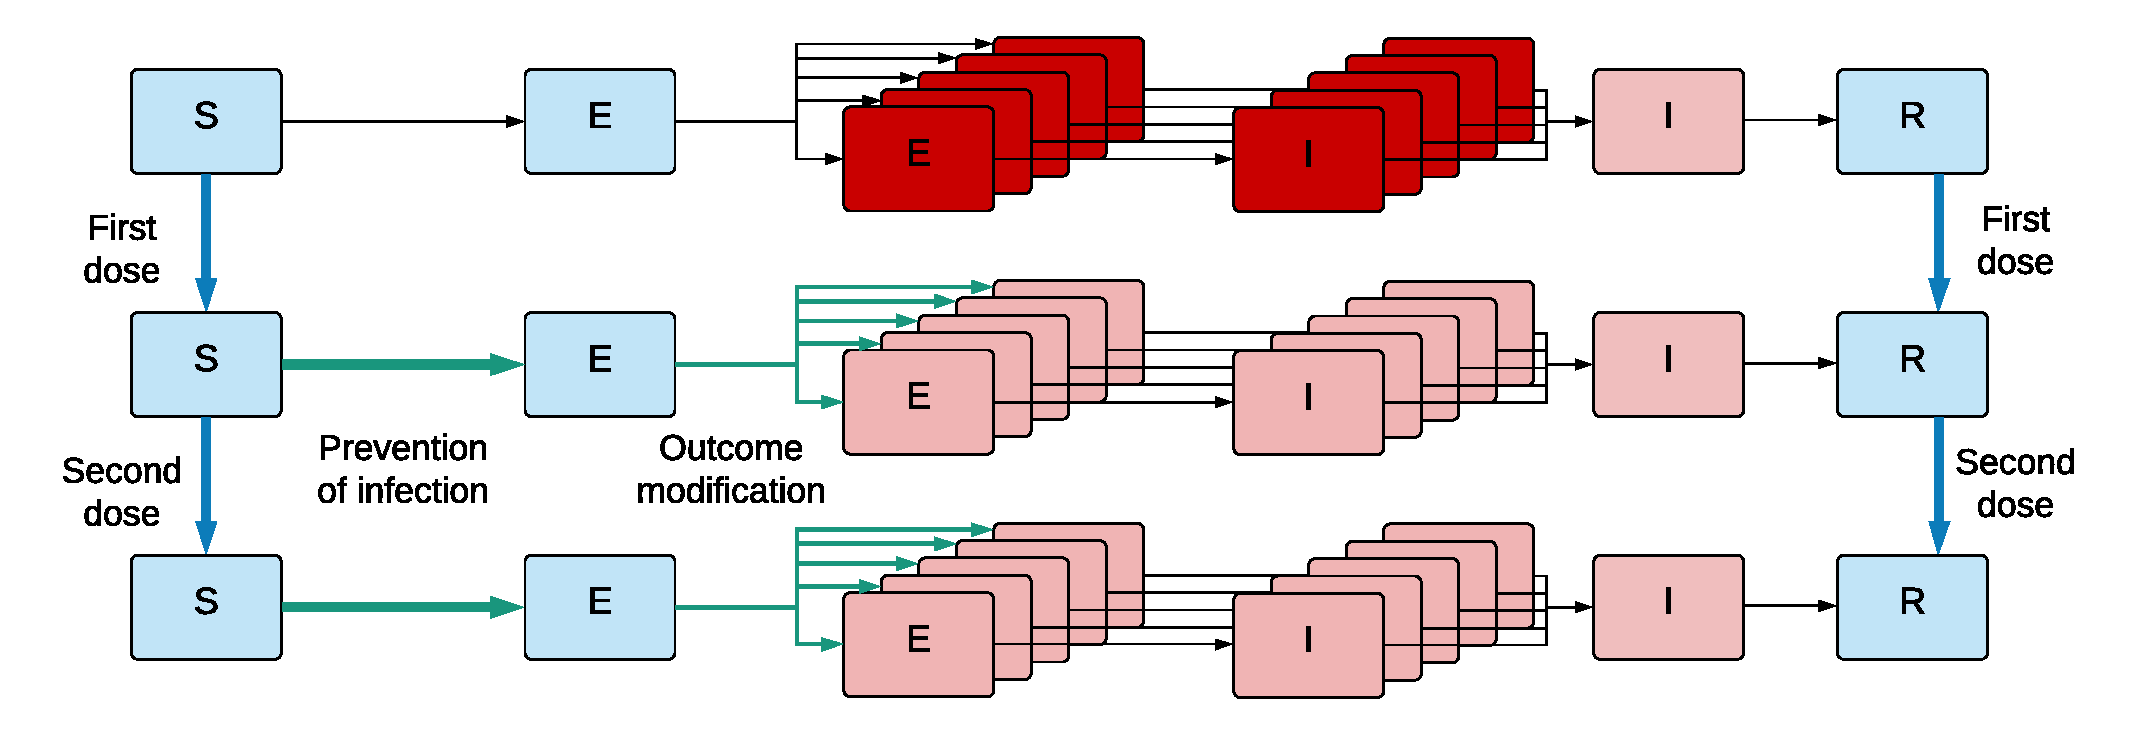
\includegraphics[width=\textwidth]{../covid_19/projects/victoria/victoria_2021/covid_19_vaccination.pdf}
   \title{Unstratified compartmental model structure.}
    \caption{\textbf{Approach to model stratification for vaccination.} Vaccination has three modelled effects: prevention of infection, reduction in severe outcomes given infection and reduction in infectiousness.}
    \label{fig:vaccination}
\end{figure}
